\documentclass[a4paper,12pt]{report} 
\usepackage[utf8x]{inputenc}
\usepackage[french]{babel}
\usepackage{mathtools}
\usepackage{amsmath, amssymb, amsfonts}
\usepackage{textcomp}
\usepackage[nointegrals]{wasysym}			% Collection de symboles mathématiques
\usepackage{ifthen}
\usepackage{tabularx}	 				% Gestion avancée des tableaux
\usepackage{longtable}		
%\usepackage{cleveref}

\usepackage{enumitem}
\usepackage{wrapfig}
%\usepackage[squaren]{SIunits}
%\usepackage[T1]{fontenc}				% Indispendable, présent dans tous les codes exemples
\usepackage[linkcolor=Indigo,colorlinks=true, citecolor=SaddleBrown, urlcolor=MidnightBlue]{hyperref} 	% Hyper ref
\usepackage{listings}					% Pour citer du code
\usepackage[justification=centering]{caption}
\usepackage{sistyle} 
\usepackage{numprint}
\usepackage{wrapfig}
\usepackage{cite}	
\usepackage{url} 					% Pour citer les sites internet dans la
%\usepackage{cleveref}
\usepackage{setspace}

\usepackage{graphicx}		 			% Inclusion des figures
\graphicspath{{./pic/}}
\usepackage[svgnames]{xcolor}			%https://www.latextemplates.com/svgnames-colors

%%% Commandes utiles définies%
\newcommand{\argmin}{\mathop{\mathrm{argmin}}}

\newcommand{\bepar}[1]{
	\left( #1 \right)  
}

\newcommand{\becro}[1]{
	\left[ #1 \right]  
}

\newcommand{\beacc}[1]{
	\left\{ #1 \right \}  
}

\newcommand{\norm}[1]{
	\left \vert \left \vert #1 \right \vert  \right \vert
}

\newcommand{\rbk}[1]{\color{red}\textit{#1} \color{black}  
}

\usepackage{listings}					% Pour citer du code
%%%%%%%%%%%%%%%%%%%
%%% Élément pour citer des codes %%%
\lstset{
language=Python,
basicstyle=\ttfamily\bfseries\small, %
identifierstyle=\bfseries\color{black}, %
keywordstyle=\color{blue}, %
stringstyle=\color{black!90}, %
commentstyle=\it\color{black!70}, %
columns=flexible, %
tabsize=4, %
extendedchars=true, %
showspaces=false, %
showstringspaces=false, % %
numberstyle=\small, %
breaklines=true, %
breakautoindent=true, %
captionpos=b,
otherkeywords={cross_val_score},
keywords=[0]{cv},
keywordstyle=[0]{\color{red}},
}
%%%%%%%%%%%%%%%%%%%%%
\title{\navy \textbf{Notes bibliographiques : \\ Utilisation de ML pour la turbulence} \color{black}}%%%%%%%%%%%%%%%%%%%%
\date{}
%\usepackage{multicol}
%\usepackage{etoolbox}
%\patchcmd{\thebibliography}{\section*{\refname}}
%    {\begin{multicols}{2}[\section*{\refname}]}{}{}
%\patchcmd{\endthebibliography}{\endlist}{\endlist\end{multicols}}{}{}
\usepackage[authoryear]{natbib}

\usepackage{geometry}
\geometry{hmargin=2cm, vmargin=2cm}

%%%%%%%%%%%%%%%%%%%%
%%% Couleurs %%%
\xdefinecolor{brick}{named}{DarkRed}
\xdefinecolor{navy}{named}{Navy}
\xdefinecolor{midblue}{named}{MidnightBlue}
\xdefinecolor{dsb}{named}{DarkSlateGray}
\xdefinecolor{dgreen}{named}{DarkGreen}
\xdefinecolor{indian}{named}{IndianRed}

%%% 	Raccourcis 	%%%
\newcommand{\keps}{$k-\varepsilon$}
\newcommand\bk{\color{black}}
\newcommand\brick{\color{brick}}
\newcommand\navy{\color{navy}}
\newcommand\midblue{\color{midblue}}
\newcommand\dsb{\color{dsb}}
\newcommand{\dgreen}{\color{dgreen}}
\newcommand{\dpurple}{\color{indian}}
\newcommand\red{\color{red}}

%%%%%%%% Cigles
\newcommand{\rap}{par rapport}
\newcommand{\cad}{c'est-à-dire}
\newcommand{\vav}{vis-à-vis}

%%%%%%%% Autres

%%%%%%%%%%%%%%%%%%%
% Syntax: \colorboxed[<color model>]{<color specification>}{<math formula>}
\newcommand*{\colorboxed}{}
\def\colorboxed#1#{%
  \colorboxedAux{#1}%
}
\newcommand*{\colorboxedAux}[3]{%
  % #1: optional argument for color model
  % #2: color specification
  % #3: formula
  \begingroup
    \colorlet{cb@saved}{.}%
    \color#1{#2}%
    \boxed{%
      \color{cb@saved}%
      #3%
    }%
  \endgroup
}

\renewcommand{\sectionmark}[1]{\markright{#1}}

\usepackage{fancyhdr}
\pagestyle{fancy}
\lhead{\textbf{Nathaniel} \brick \textbf{\textsc{Saura}}}
\rhead{\markright}
\cfoot{\thepage}
\renewcommand{\headrulewidth}{0.4pt}

\numberwithin{equation}{section} %%%% To count the equation like Section.Number

\usepackage{accents}
\newcommand{\vect}[1]{\accentset{\Rightarrow}{#1}}

\usepackage{multicol}		% Pour utiliser \hfill et découper une partie de son texte en colonnes
\setlength{\columnseprule}{0.1pt}
\def\columnseprulecolor{\color{red}}
\setlength{\columnsep}{1.5cm}

% Numéro Roman pour le texte
\makeatletter
\newcommand*{\rom}[1]{\expandafter\@slowromancap\romannumeral #1@}
\makeatother

\setlength{\parindent}{0pt}

\begin{document}

\section*{Contexte bibliographique}
\citep{ling2016reynolds} propose une architecture de NN inédite 

\begin{figure}[!ht]
	\centering
	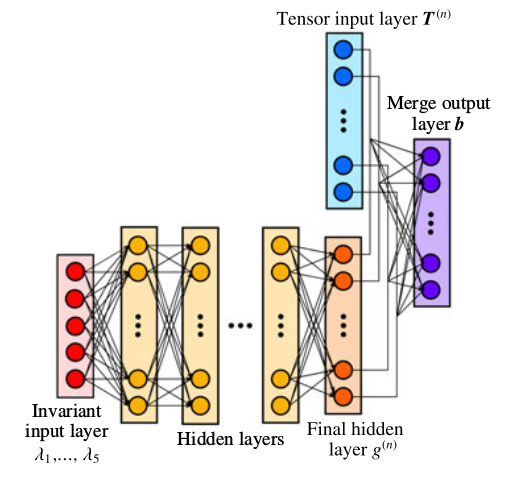
\includegraphics[scale=0.5]{TBNN.png}
	\caption{Tensor embedded NN from \citep{kutz2017deep} et \citep{ling2016reynolds}}
	\label{TBNN}
\end{figure}

\noindent Cette forme de neurones à pour but l'écriture du tenseur anisotropique comme une combinaison linéaire d'une base de tenseur bien particulière.  Les coefficients de cette combinaison sont différentes fonctions des invariants du problème. L'article se base sur les travaux de \cite{pope1975more} et de \cite{smith1965isotropic}.\\
On part de l'hypothèse de Boussinesq qui s'écrit :
\begin{equation*}
\overline{u_i' u_j'} = \frac{2}{3} k \delta_{ij} - 2 \nu_t \overline{S_{ij}}
\end{equation*}
Puis on choisit une partie déviatorique plus complexe :
\begin{equation*}
\frac{\overline{u_i' u_j'} }{2k}= \frac{1}{3} \delta_{ij} + \sum_\lambda G^\lambda T^\lambda_{ij} 
\end{equation*}
Avec une forme bien particulière pour $G$ et $T$. La première est une fonction des invariants du problème qui sont dans le cas tridimensionnel (ce sont les inputs de notre NN cf. plus loin) : 
\begin{equation*}
\mathbf{\lambda}= \left \{ Tr(\textbf{S}^2),\ Tr(\textbf{R}^2),\ Tr(\textbf{S}^3),\ Tr(\textbf{R}^2\textbf{S}),\ Tr(\textbf{R}^2 \textbf{S}^2) \right \} 
\end{equation*}

Les tenseurs considérés $\textbf{S}$ et $\textbf{R}$ sont définis par 
\begin{align*}
\textbf{S} &= \frac{k}{2\varepsilon}\left(\nabla_x\textbf{U} + \nabla^T_x\textbf{U} \right) \\[0.2cm]
\textbf{R} &= \frac{k}{2 \varepsilon}\left(\nabla_x\textbf{U} - \nabla^T_x\textbf{U} \right) 
\end{align*}

\noindent $T$ est composée de 10 tenseurs dans le cas tridimensionnel. Les 10 tenseurs proposés par \cite{pope1975more} et repris par \cite{ling2016reynolds} sont : \setlength{\columnseprule}{0pt}
\\
\vspace{-6mm}
\begin{multicols}{2}

\begin{align*}
\textbf{T}^{(1)} &= \textbf{S} \\
\textbf{T}^{(2)} &= \textbf{S}\textbf{R} - \textbf{R}\textbf{S} \\
\textbf{T}^{(3)} &= \textbf{S}^2 - \dfrac{1}{3}\, \textbf{I} \cdot \text{Tr} \left( \textbf{S}^2 \right)\\
\textbf{T}^{(4)} &= \textbf{R}^2 - \frac{1}{3}\, \textbf{I} \cdot \text{Tr} \left( \textbf{R}^2 \right)\\
\textbf{T}^{(5)} &= \textbf{R}\textbf{S}^2 - \textbf{S}^2\textbf{R}
\end{align*}

\columnbreak

\begin{align*}
\textbf{T}^{(6)} &= \textbf{R}^2\textbf{S} + \textbf{S}^2\textbf{R} - \frac{2}{3}\, \textbf{I}\cdot \text{Tr}\left(\textbf{S}\textbf{R}^2 \right) \\
\textbf{T}^{(7)} &= \textbf{R}\textbf{S}\textbf{R}^2 - \textbf{R}^2\textbf{S}\textbf{R} \\
\textbf{T}^{(8)} &= \textbf{S}\textbf{R}\textbf{S}^2 - \textbf{S}^2\textbf{R}\textbf{S} \\
\textbf{T}^{(9)} &= \textbf{R}^2\textbf{S}^2 + \textbf{S}^2\textbf{R}^2 - \frac{2}{3}\, \textbf{I}\cdot \text{Tr}\left(\textbf{S}^2\textbf{R}^2 \right)\\
\textbf{T}^{(10)} &= \textbf{R}\textbf{S}^2\textbf{R}^2 - \textbf{R}^2\textbf{S}^2\textbf{R}
\end{align*}

\end{multicols}
\vspace{2mm}

Si $T$ peut être calculé en cours de processus, apprendre $G$ est l'objectif.\\[1mm]

 Voici l'architecture du NN utilisé : 7 HL de neurones chacunes et une huitième de 10 neurones. Le learning rate $ \eta = 2.5 \times 10^{-7}$ activation \navy \textit{leakyrelu} \bk. \\

Comme on peut le voir Fig.\eqref{TBNN}, les invariants sont injectés en entrée du réseau, suivent ensuite un processus classique propre au Feed-Forward NN. La dernière HL représentera les combinaisons linéaires de coefficients et de la base $\mathbf{\Omega}$. \\
L'output s'écrira alors : $$ b_{ij} = \sum_{n=1}^{10} g^{(n)}(\lambda_1,..,\lambda_5) T_{ij}^{(n)}$$ \\

D'autres choses sont présentées dans \citep{kaandorp2018stochastic}, les problématiques sont intéressantes et doivent être prises en compte (voir intro et première section). Ils utilisent TBRF à la place de TBNN.\\

\section*{CNN}
Nous voulons utiliser les CNN pour essayer de reconstruire la totalité du Tenseur de Reynolds (ou bien sa partie déviatorique) en utilisant les CNN.\\
L'idée est d'utiliser les informations spatiales des tenseurs (et des invariants) pour pouvoir avoir une idée de la dynamique en cours et notamment du tenseur $\tau_{ij}$.\\

Comme dans l'article \citep{kaandorp2018stochastic}, l'idée ici n'est pas d'utiliser le ML comme une fin en soi mais comme un outil permettant d'améliorer un modèle. \\  L'ensemble de la dynamique du problème considéré est régie par l'équation RANS. \\

L'apport majeur de cette méthode pourrait venir de l'analyse spatiale de la solution : 
\begin{itemize}
\item Invariance galiléénnes assurées ? Si oui top, si non à quel point ? 
\item Prédiction meilleure que TBRF ou TBNN ? En quoi
\item Prédiction RANS plus proche de LES ?\\
\end{itemize}

Possibilité de mesurer la précision de l'anisotropie prédite (dans $\tau_{ij}$ ou dans $b_{ij}$ directement) et de discuter des champs turbulents : $k, \varepsilon...$.\\
Exploration des écoulements secondaires non détectés par le RANS : gradient de pressions adverses etc..\\

Cas considérés : turbulence isotrope puis anisotrope 2D ?

VAj : 
\begin{itemize}
\item GA pour optimiser taille des filtres, ensemble d'entrées
\item Autoencodage des entrées ? Plus généralement pre-processing sur les entrées : KLT (Karhunen–Loève theorem) ou PCA ? Voir autre transformation \url{http://fourier.eng.hmc.edu/e161/lectures/klt/node7.html} et \citep{berkooz1993proper}
\end{itemize} 


\subsubsection*{Nécessité}
Il nous faut un solver 2D pouvant générer des turbulences 2D anisotropes.\\
Outils de visualisation présentés dans \citep{emory2014visualizing}.
\bibliographystyle{apalike}
\bibliography{bibliotheque}

\end{document}